\input{def}

\begin{document}

\begin{center}
\large{ MATH-6890 \hspace{1in} Numerical Solutions of Waves  \hspace{1in}Fall 2016 \\ Due Monday October 24, 2016.}\end{center}
Michael Hennessey

\bigskip
\bc {\bf Problem Set 6} \ec
\benum 

\item Consider linear advection with $a>0$ as in
$$u_t+au_x=0,\;\;\; -1<x<1,\;\;\; t>0,$$
subject to initial condition $u(x,0)=u_0(x)$ and boundary condition $u(-1,t)=0.$
\benum
\item Assuming a method-of-lines time integration scheme, derive upwind finite difference approximataions to the spatial derivative term. Your derivation should use a difference of fluxes combined with a Riemann problem. Give difference approximations of formal order $\Delta x^p$ where $p=1,2,3,4.$\\

Solution:\\

We begin by writing the advection equation in conservation form
$$u_t+(au)_x=0$$
or
$$u_t+f_x=0$$
where $f=au.$ We then move the flux to the RHS of the equation and discretize to get
$$u_{tj}=-D_+F_{j-1/2}=-\frac{1}{\Delta x}[F_{j+1/2}-F_{j-1/2}].$$
where $F_{j-1/2}$ is the numerical flux function evaluated at $u^*_{j-1/2}$. We apply Riemann initial data to the advection equation above to find the state $u^*_{j-1/2}$. We let
$$u^R_{j-1/2}=u_j-\frac{\Delta x}{2}u_{xj}+\frac{\Delta x^2}{8}u_{xxj}+...$$
and
$$u^L_{j-1/2}=u_{j-1}+\frac{\Delta x}{2}u_{xj-1}+\frac{\Delta x^2}{8}u_{xxj-1}+...$$
for the Riemann problem
$$u_t+(au)_x=0$$
$$u(x,0)=\left\{\begin{array}{cc}u^R_{j-1/2},&x>x_{j-1/2}\\ u^L_{j-1/2},&x<x_{j-1/2}\end{array}\right..$$
Then, the star state $u^*_{j-1/2}$ is the solution of the Riemann problem at $x=x_{j-1/2}$ at time $t>0.$ Since the PDE describes linear advection to the right of the domain, we have $u^*_{j-1/2}=u^L_{j-1/2}.$ Note, this result holds for all $j$. Therefore, our flux will always be evaluated to the left. For the 1st and 2nd order accurate code, we can simply make the choice that the numerical flux and the flux are equivalent, and get:
$$u_{tj}=-\frac{1}{\Delta x}[F_{j+1/2}-F_{j-1/2}]=-\frac{a}{\Delta x} [u^L_{j+1/2}-u^L_{j-1/2}].$$
Once this choice is made, the order of accuracy is entirely dependent on how we define $u^L_{j\pm 1/2}.$\\
To get 1st order accuracy $(p=1)$, we simply let $u^L_{j-1/2}=u_{j-1}.$ Then the first order accurate scheme is
$$u_{tj}=\frac{-a}{\Delta x}[u_j-u_{j-1}].$$
To get 2nd order accuracy $(p=2)$, we take another term in the series for $u^L_{j-1/2}$ and get
$$u^L_{j-1/2}=u_{j-1}+\frac{\Delta x}{2}u_{xj-1}.$$
We can either use a centered difference scheme for $u_x$ or we can use an upwind discretization to get the appropriate order of accuracy. I will choose to use centered discretizations from here on out. Using the 1st order centered difference we get
$$\frac{\Delta x}{2}u_{xj}\approx \frac{1}{4}[u_{j+1}-u_{j-1}].$$
Then the 2nd order scheme takes the form
$$u_{tj}=\frac{-a}{\Delta x}(u_j-u_{j-1}+\frac{1}{4}[u_{j+1}-u_j-u_{j-1}+u_{j-2}])=\frac{-a}{4\Delta x}[u_{j+1}+3 u_j-5u_{j-1}+u_{j-2}].$$
The 3rd order scheme requires a more accurate discretization of the numerical flux function $F_{j+1/2}$, the 2nd order 1st derivative and the 2ndt order 2nd derivative, which we take
$$F_{j+1/2}=f_{j+1/2}-\frac{\Delta x^2}{24}f_{xxj+1/2},$$
$$\frac{\Delta x}{2}u_{xj}\approx \frac{1}{4}[u_{j+1}-u_{j-1}],$$
$$\frac{\Delta x^2}{8}u_{xxj}\approx\frac{1}{8}[u_{j+1}-2u_{j}+u_{j-1}].$$
Then the scheme is
\begin{align*}
u_{tj}&=\frac{-a}{\Delta x}(u_j-u_{j-1}+\frac{1}{4}[u_{j+1}-u_j-u_{j-1}+u_{j-2}]+\frac{1}{12}[u_{j+1}-3u_j+3u_{j-1}-u_{j-2}])\\
&=\frac{-a}{6\Delta x}[2u_{j+1}+3u_{j}-6u_{j-1}+u_{j-2}].
\end{align*}
Lastly, the 4th order scheme requires the 4th order first derivative, the 2nd order 2nd derivative, and no 3rd derivative (due to cancellation), along with the same numerical flux as above. These take the forms:
$$\frac{\Delta x}{2}u_{xj}\approx\frac{1}{12}[-u_{j+2}+8u_{j+1}-8u_{j-1}+u_{j-2}],$$
$$\frac{\Delta x^2}{8}u_{xxj}\approx\frac{1}{8}[u_{j+1}-2u_{j}+u_{j-1}].$$
Then the scheme is
\begin{align*}
u_{tj}=&\frac{-a}{\Delta x}(u_j-u_{j-1}+\frac{1}{24}[-u_{j+2}+9u_{j+1}-8u_j-8u_{j-1}+9u_{j-2}-u_{j-3}]\\
&+\frac{1}{12}[u_{j+1}-3u_j+3u_{j-1}-u_{j-2}]\\
=&\frac{-a}{24\Delta x}[-u_{j+2}+11u_{j+1}+10u_j-26u_{j-1}+7u_{j-2}-u_{j-3}].
\end{align*}


\item Plot the real and imaginary parts of the symbol to the difference approximations from (1a).\\


We begin writing the symbols by making the ansatz $u_j=e^{ikx_j}.$ Then the symbols for the approximations in increasing order of accuracy are:
$$-ai\xi=-a[1-e^{-i\xi}],$$
$$-ai\xi=\frac{-a}{4}[e^{i\xi}+3-5e^{-i\xi}+e^{-2i\xi}],$$
$$-ai\xi=\frac{-a}{6}[2e^{i\xi}+3-6e^{-i\xi}+e^{-2i\xi}],$$
$$-ai\xi=\frac{-a}{24}[-e^{2i\xi}+11e^{i\xi}+10-226e^{-i\xi}+7e^{-2i\xi}-e^{-3i\xi}],$$
where $\xi=k\Delta x.$ The plot of these symbols is included here with $a=1.$
\begin{figure}[h]
\centering
\includegraphics[width=3in]{realsym}
\includegraphics[width=3in]{imsym}\\
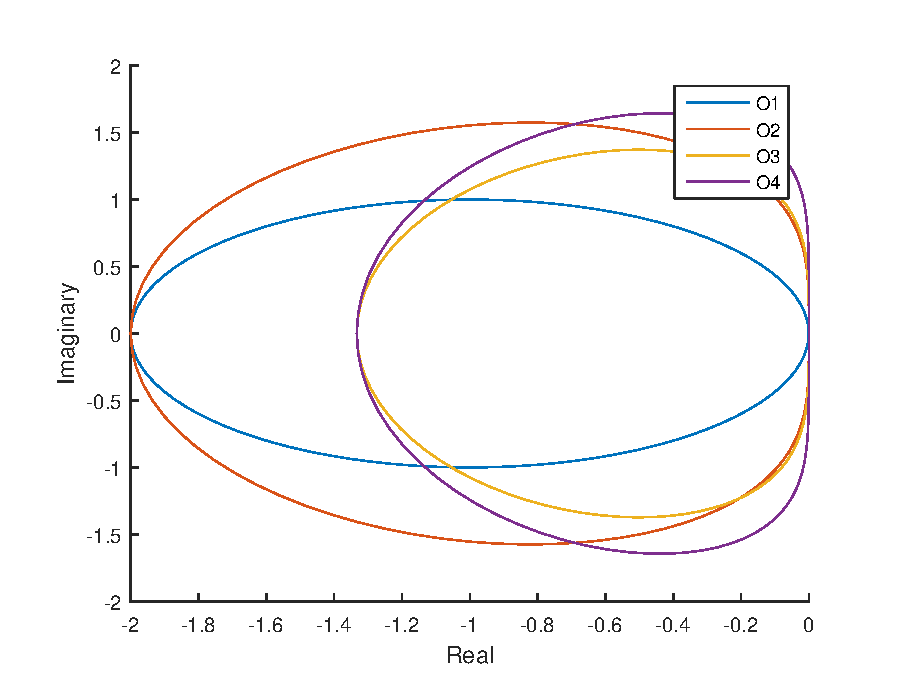
\includegraphics[width=3in]{sym}
\end{figure}

\item Using RK-4, demonstrate the design order of accuracy in $L_1$ and $L_\infty$ for smooth initial conditions.\\

For initial data, we choose 
$$u(x,0)=u_0(x)=\left\{\begin{array}{cc}0,&x<-\pi/4\\ cos^{5}(2x),&x\geq -\pi/4\end{array}\right..$$
 Then the exact solution of the advection PDE with this initial data is
$$u_e(x,t)=u_0(x-at).$$
We compare our numerical method against this exact solution.\\

The numerical scheme then is RK-4 in time with the above difference schemes in space. We use the grid $x_j=j\Delta x, j=1,...,N$ where $\Delta x=[1-(-1)]/N$ and $N$ is the number of points in the interior of the domain. Initialization is trivial, but treating the boundary requires its own discussion. For the 1st order spatial discretization, we need 1 ghost point at the left, i.e., $u_0$ (due to only using backward difference), for the 2nd order spatial discretization we need 2 ghost points at the left, $u_0,u_{-1}$, etc... We define our ghost points by examing our Dirichlet condition $u(-1,t)=0.$ We differentiate this condition once in time for each order of accuracy to get the appropriate compatibility boundary conditions. These are summaried here:
\begin{align*}
O(\Delta x):&\;\;\; u_{0}=u_1,\\
O(\Delta x^2):&\;\;\; u_0=u_1,\;\; u_{-1}=u_1,\\
O(\Delta x^3):&\;\;\; u_0=u_1,\;\; u_{-1}=u_1,\;\; u_{-2}=u_1,\\
O(\Delta x^4):&\;\;\; u_0=u_1,\;\; u_{-1}=u_1,\;\; u_{-2}=u_1,\;\; u_{-3}=u_1.
\end{align*}
To define the ghost points on the right for the centered schemes, we need to extrapolate. These points are given here:
\begin{align*}
O(\Delta x^2):&\;\;\; u_{N+1}=3u_N-3u_{N-1}+u_{N-2},\;\; u_{N+2}=3u_{N+1}-3u_N+u_{N-1},\\
O(\Delta x^3):&\;\;\; u_{N+1}=4u_N-6u_{N-1}+4u_{N-2}-u_{N-3},\;\; u_{N+2}=4u_{N+1}-6u_N+4u_{N-1}-u_{N-2},\\
&\;\;\;u_{N+3}=4u_{N+2}-6u_{N+1}+4u_{N}-u_{N-1}\\
O(\Delta x^4):&\;\;\; u_{N+1}=4u_N-6u_{N-1}+4u_{N-2}-u_{N-3},\;\; u_{N+2}=4u_{N+1}-6u_N+4u_{N-1}-u_{N-2},\\
&\;\;\;u_{N+3}=4u_{N+2}-6u_{N+1}+4u_{N}-u_{N-1},\;\;\; u_{N+4}=4u_{N+3}-6u_{N+2}+4u_{N+1}-u_{N}\\
\end{align*}

A convergence plot is included at the beginning of the next page for each difference scheme. The code is located at the end of this document.

\begin{figure}[h]
\centering
\includegraphics[width=3in]{1conv}
\includegraphics[width=3in]{2conv}\\
\includegraphics[width=3in]{3conv}
\includegraphics[width=3in]{4conv}
\caption{Convergence Plot with Smooth Initial Data}
\end{figure}

\item Again using RK-4 as a time integration scheme, demonstrate $L_1$ convergence at (or near) the rate $p/(p+1)$ for an initial condition with a discontinuity. Also discuss the nature of the discrete approximations paying particular attention to behavior at different $p.$\\

We use top-hat initial data $u_0(x)$ to inspect convergence for the discontinuous case, where $u_0$ is defined
$$u(x,0)=u_0(x)=\left\{\begin{array}{cc}0,&x<-3/4\\ 1,&-3/4<x<1/4\\0,&x>1/4\end{array}\right.$$
A convergence plot is included on page 6.
\begin{figure}[h]
\centering
\includegraphics[width=3in]{50conv}
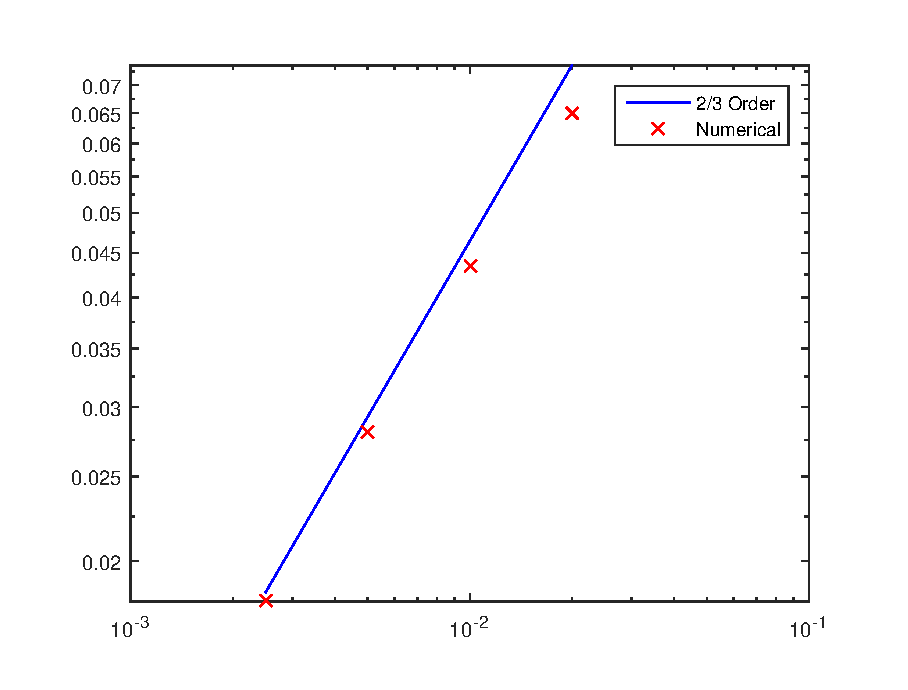
\includegraphics[width=3in]{67conv}\\
\includegraphics[width=3in]{75conv}
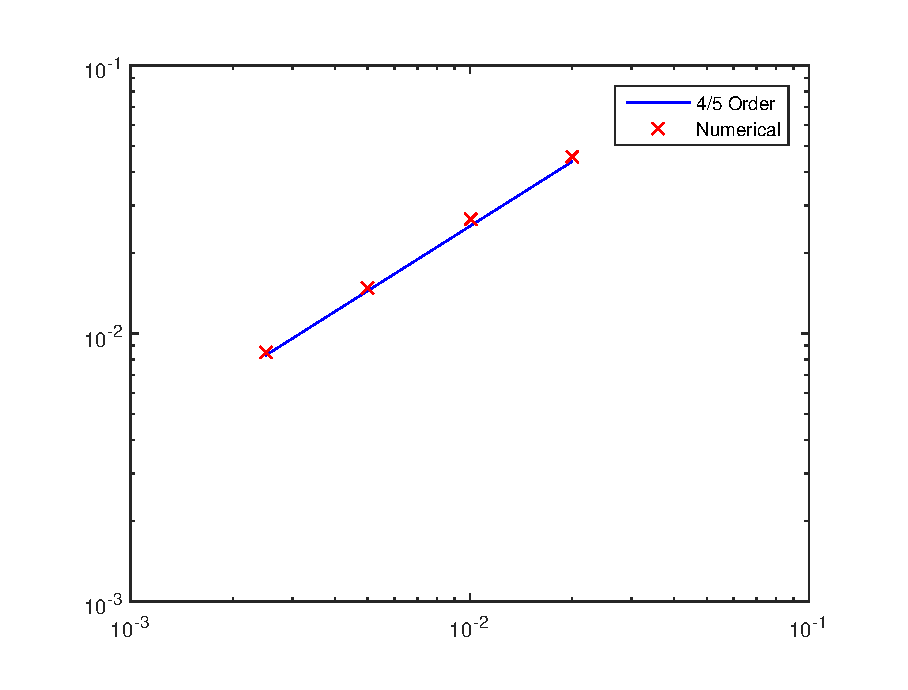
\includegraphics[width=3in]{80conv}
\caption{Convergence Plot with Nonsmooth Initial Data}
\end{figure}

A snapshot of each solution at the final time of integration is included on page 7. The 1st order accurate code very clearly bisects the shockwaves and is clearly area preserving, though it does seem awfully dispersive. The 2nd order accurate code bisects the wave well and is smooth on the left, but overshoots the wave on the right which introduces some oscillations. The 3rd order accurate code bisects the wave clearly, but overshoots on both sides to seemingly the same degree and introduces oscillations on both sides. The 4th order accurate code behaves similarly as the 3rd order accurate code, but the overshot in height is significantly worse than the 3rd order's. 
\begin{figure}[h]
\centering
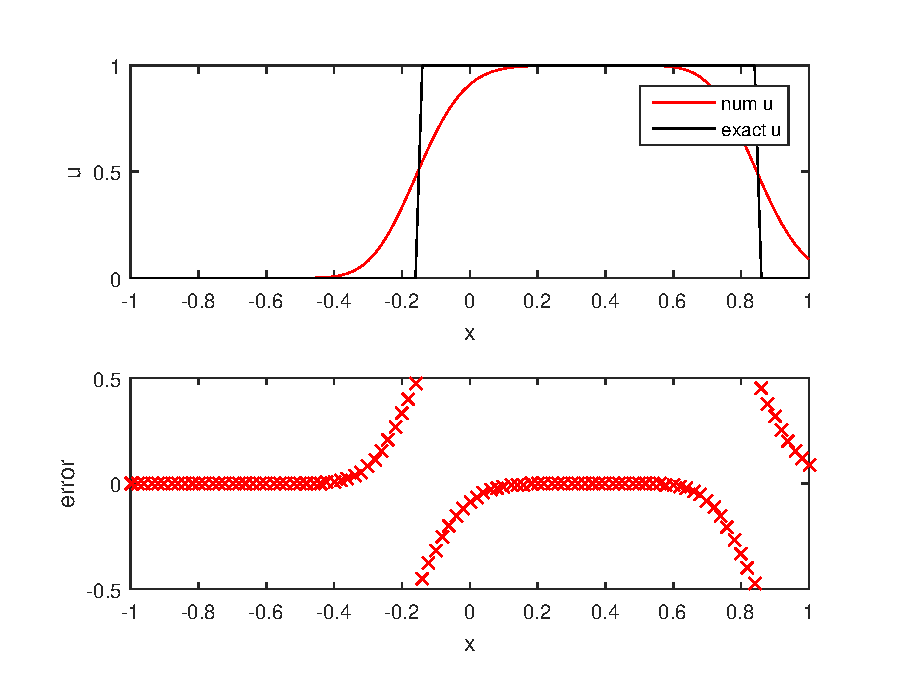
\includegraphics[width=3in]{unsmooth1}
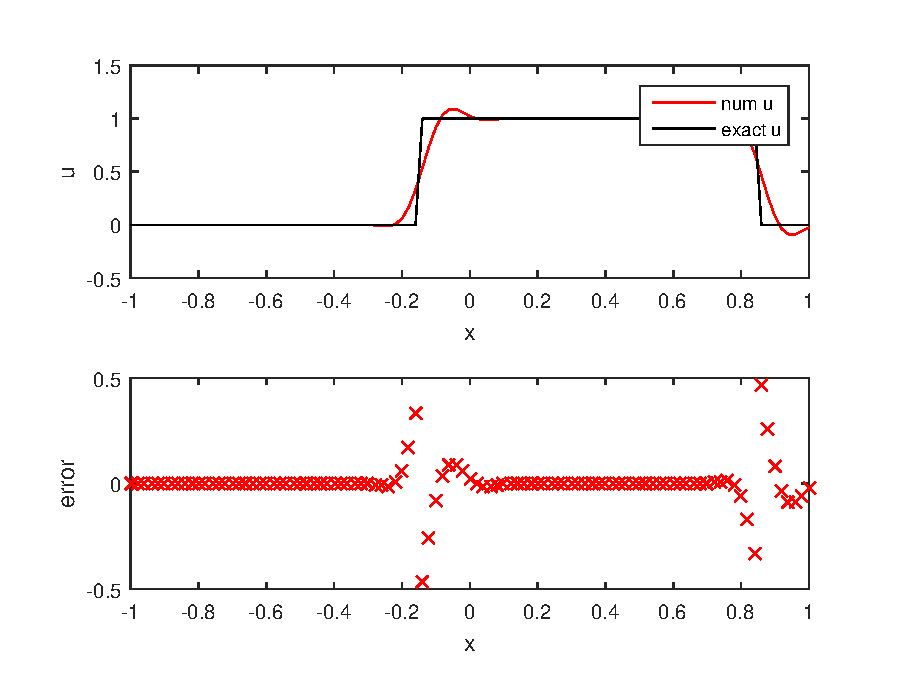
\includegraphics[width=3in]{unsmooth2}\\
\includegraphics[width=3in]{unsmooth3}
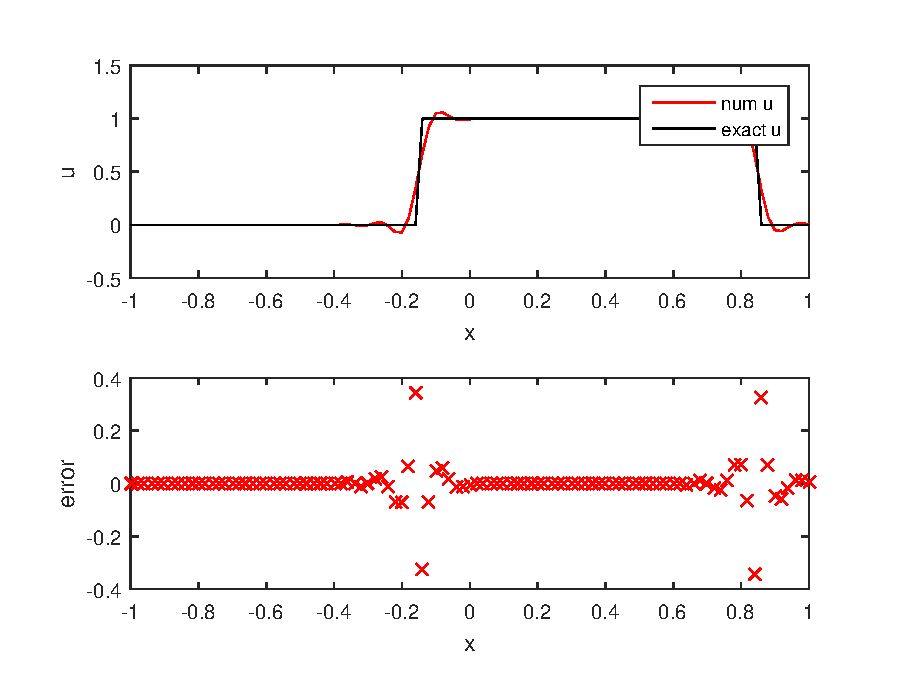
\includegraphics[width=3in]{unsmooth4}
\caption{Advection Solution Behavior at $t_f=.3.$ Top left is 1st order accurate, top right is 2nd order accurate, bottom left is 3rd order accurate, bottom right is 4th order accurate.}
\end{figure}



\item Apply Richardson extrapolation to estimate convergence rates for the problems discussed in (1c) and (1d). For both classes of ICs you should report both $L_1$ and $L_\infty$ convergence rates.\\

We apply Richardson extrapolation by assuming the numerical solution to the differential equation takes the form 
$$u_h=u_{ex}+ch^p,$$
and comparing the ratio of the difference between three consecutive approximations and their discretization variable $h=\Delta x.$ This takes the form
$$\frac{||u_1-u_0||}{||u_2-u_1||}=\frac{|h_1^p-h_0^p|}{|h_2^p-h_1^p|}.$$
We can choose $\alpha^2 h_2=\alpha h_1=h_0$ to simplify this equation and solve for $p$:
$$p=\frac{\log\left(\frac{||u_1-u_0||}{||u_2-u_1||}\right)}{\log\left(\frac{1}{\alpha}\right)}.$$ 
For this test, I take 300 points initially, then 600, then 1200 ($\alpha=2$) up to $t_f=.3$.
The results of running this test may be found in the table below.
\begin{table}[h]
\centering
\begin{tabular}{c|c|c|c|c}
\hline
\multicolumn{4}{c}{Order  \hspace{.5cm}  Smooth Data \hspace{.5cm}     Nonsmooth Data}\\
\hline
&1-norm&$\infty$-norm&1-norm&$\infty$-norm\\
1&0.9675&0.9629&0.5111&0.1343\\
2&1.9968&2.0021&0.6532&-0.0713\\
3&2.9996&2.9994&0.7268&-0.1304\\
4&4.0416&4.0380&0.8605&0.0816\\
\hline
\end{tabular}
\end{table}

\eenum
\vspace{1.1in}
\item Given PS3 number 2 and 3, and PS4 number 4 you now have second and fourth-order accurate codes for the initial-boundary value problem
$$ u_{tt}=c^2(u_{xx}+u_{yy}),\;\; 0<x<\pi,\;\;0<y<\pi,\;\; t>0$$
with initial and boundary conditions
\begin{align*}
u(0,y,t)=u(\pi,y,t)&=0\\
u_y(x,0,t)=u_y(x,\pi,t)&=0\\
u(x,y,0)&=u_0(x,y)\\
u_t(x,y,0)&=0.
\end{align*}
\benum
\item Use Richardson extrapolation to demonstrate the expected convergence rates for an appropriately smooth $u_0$. You can take inspiration from the IC used for (1c) above, and be sure to run the problem long enough in time so that the waves interact with the boundaries.\\

Solution:
We run the wave equation in 2D with initial condition 
$$u(x,y,0)=u_0(x,y)=\left\{\begin{array}{cc}0,&x,y<\pi/4\\ (\cos(2x)\cos(2y))^5,&\pi/4<x,y<3\pi/4\\0,&x,y>3\pi/4\end{array}\right..$$
Then, with Richardson extrapolation worked out as before, we get the results in the table found on the next page, when run with 30$\times$ 30 pts, then $60\times60$ pts, then $120\times 120$ pts ($\alpha=2)$ up to $t_f=4$ (to ensure interaction with the boundary).
\begin{table}[h]
\centering
\begin{tabular}{c|c|c}
\hline
Order&1-norm&$\infty$-norm\\
2&1.9904&2.2759\\
4&3.8835&3.9812\\
\hline
\end{tabular}
\caption{2-D Wave Richardson Extrapolation Results for Smooth Initial Data}
\end{table}
\item Use Richardson extrapolation to explore the convergence rates for $u_0$ with a kink, i.e. a triangle wave.\\

Using the exact same set up as in part (a), but with initial condition
$$u_0(x,y)=\left\{\begin{array}{cc}(4x-\pi)(4y-\pi),&\pi/4<x,y<\pi/2\\ (-4x+3\pi)(-4y+3\pi),&\pi/2<x,y<3\pi/4\\0,&\text{else}\end{array}\right..$$
The results for this test are found in the table presented here.
\begin{table}[h]
\centering
\begin{tabular}{c|c|c}
\hline
Order&1-norm&$\infty$-norm\\
2&0.9233&1.2324\\
4&1.1630&0.6064\\
\hline
\end{tabular}
\end{table}

\item Use Richardson extrapolation to explore the convergence rates for $U_0$ with a jump, i.e. a top hat.\\
Here we use initial data
$$u_0(x,y)=\left\{\begin{array}{cc}1&\pi/3<x,y<2\pi/3 \\0,&\text{else}\end{array}\right..$$
The results for this test may be found here. Unfortunately, I did not have time to implement this code in the C-architechture so that the convergence test may be run on larger grids to get better $p$ values.
\begin{table}[h]
\centering
\begin{tabular}{c|c|c}
\hline
Order&1-norm&$\infty$-norm\\
2&0.3429&-0.0444\\
4&0.5127&0.1177\\
\hline
\end{tabular}
\end{table}
\eenum

\item Give a 1-page proposal for the project that you plan to pursue.
\eenum
\pagebreak
\bc {\bf Code Appendix} \ec
Conservative Advection Solver:
\begin{lstlisting}[frame=single]
function [dx,err,err1,data,x]=consAdvSolvV2(a,N,xa,xb,cfl,tf,order,iPlot)
%Determines Numerical Solution to the Conservation Law u_t+f(u)_x=0
err=0;
%% Initialize Variables
%Number of ghost points
if order==1
    ng=1;
elseif order==2
    ng=2;
elseif order==3
    ng=3;
elseif order==4
    ng=4;
end

%% Grid size and other grid quantities
dx=(xb-xa)/N;
dt=cfl*dx/a;
Nt=ceil(tf/dt);
dt=tf/Nt;

Ntot=N+1+2*(ng);

%% First and last interior grid points
ia=ng+1;
ib=Ntot-ng;

x = linspace(xa-ng*dx,xb+(ng)*dx,Ntot);

%% Set initial conditions
t=0;
u=setICs(x,ia,ib);
%% Main loop
for n=1:Nt
    %% Set BCs on current time step
    u=setBCs(u,ia,ib,order);
    %% Compute RK-4 constants
    [k1]=computeK(u,a,ia,ib,dx,order);
    %ua=u+dt*.5*k1;
    [ua]=setBCs(u+dt*.5*k1,ia,ib,order);
    [k2]=computeK(ua,a,ia,ib,dx,order);
    %ub=u+dt*.5*k2;
    [ub]=setBCs(u+dt*.5*k2,ia,ib,order);
    [k3]=computeK(ub,a,ia,ib,dx,order);
    %uc=u+dt*k3;
    [uc]=setBCs(u+dt*k3,ia,ib,order);
    [k4]=computeK(uc,a,ia,ib,dx,order);
    %Update solution
    for i=ia:ib
        u(i)=u(i)+dt/6*(k1(i)+2*k2(i)+2*k3(i)+k4(i));
    end
    
    %Update time
    t=t+dt;
    
    %% Check error
    [ue]=uex(x-a*t);
    ind=ia:ib;
    err=max(abs(u(ind)-ue(ind)));
    %% Plot Solution
    if iPlot==1
        plotStuff(x,u,ue,ind);
    end
end
err1=0;
for i=1:N
    err1=dx*abs(u(i)-ue(i))+err1;
end

data=u;
%% Initial Condition Functions
    function z=f(x)
%         if x<-pi*.25
%             z=0;
%         else
%             z=(cos(2*x)).^5;
%         end
        if x>-.75&&x<=.25
            z=1;
        else
            z=0;
        end
    end

%Sets condition at t=0
    function u=setICs(x,ia,ib)
        u=zeros(size(x));
        for j=ia:ib
            u(j)=f(x(j));
        end
    end

%% Exact Solution
    function z=uex(x)
        z=zeros(1,numel(x));
        for j=1:numel(x)
            z(j)=f(x(j));
        end
    end

%% Boundary Condition Function
    function u=setBCs(u,ia,ib,order)
        %u(ia)=0;
        if order==1
            u(ia-1)=u(ia);
            %u(ib+1)=-u(ib-1);
        elseif order==2
            u(ia-2)=u(ia);
            u(ia-1)=u(ia);
            u(ib+1)=3*u(ib)-3*u(ib-1)+u(ib-2);
            u(ib+2)=3*u(ib+1)-3*u(ib)+u(ib-1);
        elseif order==3
            u(ia-3)=u(ia);
            u(ia-2)=u(ia);
            u(ia-1)=u(ia);
            u(ib+1)=4*u(ib)-6*u(ib-1)+4*u(ib-2)-u(ib-3);
            u(ib+2)=4*u(ib+1)-6*u(ib)+4*u(ib-1)-u(ib-2);
            u(ib+3)=4*u(ib+2)-6*u(ib+1)+4*u(ib)-u(ib-1);
        elseif order==4
            u(ia-4)=u(ia);
            u(ia-3)=u(ia);
            u(ia-2)=u(ia);
            u(ia-1)=u(ia);
            u(ib+1)=4*u(ib)-6*u(ib-1)+4*u(ib-2)-u(ib-3);
            u(ib+2)=4*u(ib+1)-6*u(ib)+4*u(ib-1)-u(ib-2);
            u(ib+3)=4*u(ib+2)-6*u(ib+1)+4*u(ib)-u(ib-1);
            u(ib+4)=4*u(ib+3)-6*u(ib+2)+4*u(ib+1)-u(ib);
        end
    end
%% Compute RK-4 Coefficient Function
    function K=computeK(u,a,ia,ib,dx,order)
        K=zeros(size(u));
        for j=ia:ib
            if order==1
                flp=u(j);
                flm=u(j-1);
                flpxx=0;
                flmxx=0;
            elseif order==2
                uxp=(u(j+1)-u(j-1))/(2*dx);
                uxm=(u(j)-u(j-2))/(2*dx);
                flp=u(j)+dx*uxp/2;
                flm=u(j-1)+dx*uxm/2;
                flpxx=0;
                flmxx=0;
            elseif order==3
                uxp=(u(j+1)-u(j-1))/(2*dx);
                uxm=(u(j)-u(j-2))/(2*dx);
                uxxp=(u(j+1)-2*u(j)+u(j-1))/(dx^2);
                uxxm=(u(j)-2*u(j-1)+u(j-2))/(dx^2);
                flp=u(j)+dx*uxp/2+dx^2*uxxp/8;
                flm=u(j-1)+dx*uxm/2+dx^2*uxxm/8;
                flpxx=uxxp;
                flmxx=uxxm;
            elseif order==4
                uxxp=(u(j+1)-2*u(j)+u(j-1))/(dx^2);
                uxxm=(u(j)-2*u(j-1)+u(j-2))/(dx^2);
                uxp=(-u(j+2)+8*u(j+1)-8*u(j-1)+u(j-2))/(12*dx);
                uxm=(-u(j+1)+8*u(j)-8*u(j-2)+u(j-3))/(12*dx);
                flp=u(j)+dx*uxp/2+dx^2*uxxp/8;
                flm=u(j-1)+dx*uxm/2+dx^2*uxxm/8;
                flpxx=uxxp;
                flmxx=uxxm;
            end
            K(j)=-a*(flp-dx^2*flpxx/24-(flm-dx^2*flmxx/24))/dx;
        end
    end
%% Plot Function
    function plotStuff(x,u,ue,ind)
        subplot(2,1,1)
        plot(x(ind),u(ind),'rx',x(ind),ue(ind),'k-')
        xlabel('x')
        ylabel('u')
        legend('num u','exact u')
        subplot(2,1,2)
        plot(x(ind),u(ind)-ue(ind),'rx')
        xlabel('x')
        ylabel('error')
        drawnow
        pause
    end    
end
\end{lstlisting}
\pagebreak
Richardson Tester
\begin{lstlisting}[frame=single]
%% Richardson Test
if 2==2
    order=4
    N0=350;
    alpha=2;
    N1=N0;
    N2=N0*alpha;
    N3=N0*alpha^2;
    [dx1,~,~,data1,x1]=consAdvSolvV2(a,N1,-1,1,.8,.2,order,0);
    [dx2,~,~,data2,x2]=consAdvSolvV2(a,N2,-1,1,.8,.2,order,0);
    [dx3,~,~,data3,x3]=consAdvSolvV2(a,N3,-1,1,.8,.2,order,0);
    if abs(dx1-dx2*alpha)>1e-13
        fprintf('dx1 and dx2 wrong')
        return
    end
    if abs(dx2-dx3*alpha)>1e-13
        fprinf('dx2 and dx3 wrong')
        return
    end
        
    norm1=0;
    norm2=0;
    mnorm1=0;
    mnorm2=0;
    for i=1:N1
        for j=1:N2
            if abs(x1(i)-x2(j))<1e-13
                norm1=dx1*abs(data1(i)-data2(j))+norm1;
                mnorm1=max(abs(data1(i)-data2(j)),mnorm1);
            end
        end
    end
    
    for i=1:N1
        for j=1:N2
            for k=1:N3
                if abs(x2(j)-x3(k))<1e-13 && abs(x1(i)-x3(k))<1e-13
                    norm2=dx1*abs(data2(j)-data3(k))+norm2;
                    mnorm2=max(abs(data2(j)-data3(k)),mnorm2);
                end
            end
        end
    end
    p=log(norm2/norm1)/log(1/alpha)
    pmax=log(mnorm2/mnorm1)/log(1/alpha)
end
\end{lstlisting}
\end{document}